\chapter{Magic Formula Pacejka}
\label{Ch:MagicFormula}
%
The model used in this thesis for the forces is the same proposed for motorcycles by Hans Pacejka.\cite{pacejka2012tire} The data for the tyre are taken from the example chapter 12 of "Vehicle and Tyre Dynamics" and other publications.\cite{sharp2004advances,sharp2014method}
%
\section{Longitudinal force}
%
\begin{figure}%[hbt]
    \begin{subfigure}{.5\linewidth}
        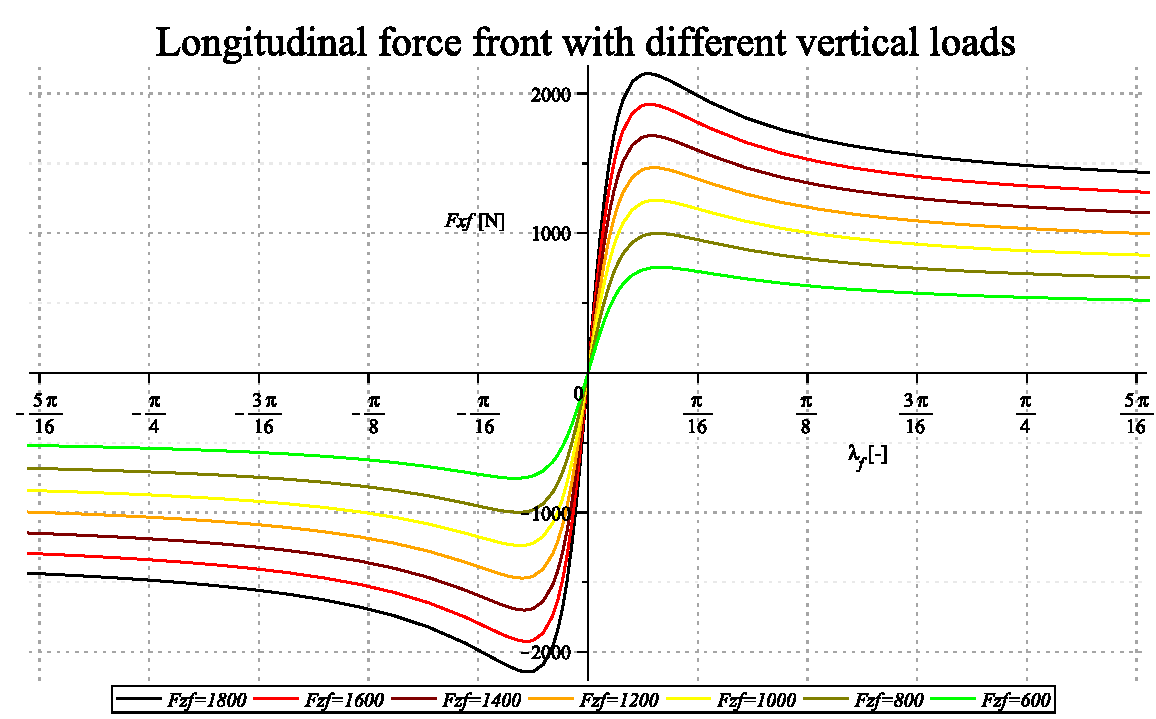
\includegraphics[width=\linewidth]{Pacejka/LongFrontFz.pdf}
        \caption{}
        \label{fig:long1a}
    \end{subfigure}%
    \begin{subfigure}{.5\linewidth}
        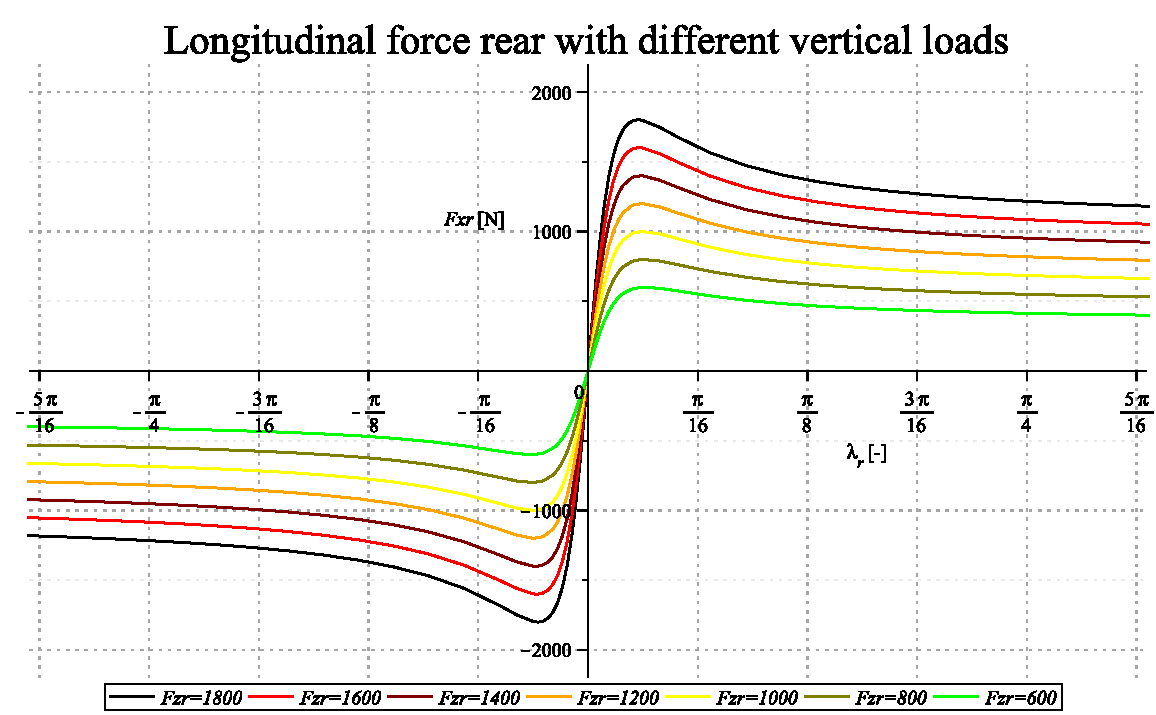
\includegraphics[width=\linewidth]{Pacejka/LongRearFz.pdf}
        \caption{}
        \label{fig:long1b}
    \end{subfigure}
    \caption{Graphs of the longitudinal force for front and rear wheel}
\end{figure}
%
%
The longitudinal forces are described by the following relationship where $\lambda$ represent the longitudinal slip defined in the previous chapters. Usually longitudinal slip is small or at list constrained to be small to have good performances.
%
\begin{equation}
    \begin{array}{l}
        Fxf = Dx_f  \sin( Cx_f  \arctan(Bx_f  \lambda_{x_f} + SHx_f  ) ) + SVx_f\\
        Fxr = Dx_r  \sin( Cx_r  \arctan(Bx_r  \lambda_{x_r} + SHx_r  ) ) + SVx_r
    \end{array}
\end{equation}
%
Here, the time dependency is being dropped to have a lighter notation. This formula comes from the book "Tire and Vehicle Dynamics" $3^{rd}$ edition\cite{pacejka2012tire} which is more compact with respect to the one of the older version\cite{pacejka2006tyre}.
All parameters inside are function of other variables with the following definition.
%
% \begin{equation}
%     \left[ \begin {array}{c} {\it dfz}_{f} =\frac{{\it Fzf} \left(t 
% \right)-{\it Fz0} }{{\it Fz0} }\\ \lambda_{x_{f}} =
% \lambda_{f} \left(t \right)+{\it SHx}_{f} \\ {\it Cx
% }_{f} =\lambda_{C_{x_{f}}} ~{\it pCx1}_{f} \\ {\it 
% Dx}_{f} ={\it Fzf} \left(t \right)~\mu_{x_{f}} \\ 
% \mu_{x_{f}} =\left({\it dfz}_{f} ~{\it pDx2}_{f} +{\it pDx1}_{f} 
% \right)~\lambda_{\mu_{x_{f}}} \\ {\it Ex}_{f} =
% \lambda_{E_{x_{f}}} ~\left(1-{\it pEx4}_{f} \right)~\left({\it dfz}_{f
% } ^{2}~{\it pEx3}_{f} +{\it dfz}_{f} ~{\it pEx2}_{f} +{\it pEx1}_{f} 
% \right)\\ {\it Kx}_{\lambda_{f}} =\lambda_{K_{x_{f}}
% } ~e^{{\it dfz}_{f} ~{\it pKx3}_{f} }~\left({\it dfz}_{f} ~{\it pKx2}_
% {f} +{\it pKx1}_{f} \right)~{\it Fzf} \left(t \right)
% \\ {\it Bx}_{f} =\frac{{\it Kx}_{\lambda_{f}} }{{
% \it Dx}_{f} ~{\it Cx}_{f} +\epsilon_{x_{f}} }\\ {
% \it SHx}_{f} =0\\ {\it SVx}_{f} =0\end {array}
%  \right] 
% \end{equation}
% %
% \begin{equation}
%     \left[ \begin {array}{c} {\it dfz}_{r}={\frac {{\it Fzr} \left( t
%  \right) -{\it Fz0}}{{\it Fz0}}}\\ \lambda_{x_{r}}=
% \lambda_{r} \left( t \right) +{\it SHx}_{r}\\ {\it 
% Cx}_{r}=\lambda_{C_{x_{r}}}\,{\it pCx1}_{r}\\ {\it 
% Dx}_{r}={\it Fzr} \left( t \right) \mu_{x_{r}}\\ \mu
% _{x_{r}}= \left( {\it dfz}_{r}\,{\it pDx2}_{r}+{\it pDx1}_{r} \right) 
% \lambda_{\mu_{x_{r}}}\\ {\it Ex}_{r}=\lambda_{E_{x_{
% r}}}\, \left( 1-{\it pEx4}_{r} \right)  \left( {{\it dfz}_{r}}^{2}{
% \it pEx3}_{r}+{\it dfz}_{r}\,{\it pEx2}_{r}+{\it pEx1}_{r} \right) 
% \\ {\it Kx}_{\lambda_{r}}=\lambda_{K_{x_{r}}}\,{
% {\rm e}^{{\it dfz}_{r}\,{\it pKx3}_{r}}} \left( {\it dfz}_{r}\,{\it 
% pKx2}_{r}+{\it pKx1}_{r} \right) {\it Fzr} \left( t \right) 
% \\ {\it Bx}_{r}={\frac {{\it Kx}_{\lambda_{r}}}{{
% \it Cx}_{r}\,{\it Dx}_{r}+\epsilon_{x_{r}}}}\\ {\it 
% SHx}_{r}=0\\ {\it SVx}_{r}=0\end {array} \right]
% \end{equation}
%
\begin{equation}
\left[ \begin {array}{c} \displaystyle {\it dfz}_{i} =\frac{{\it Fzi} \left(t 
\right)-{\it Fz0} }{{\it Fz0} }\\ \lambda_{x_{i}} =
\lambda_{i} \left(t \right)+{\it SHx}_{i} \\ {\it Cx
}_{i} =\lambda_{C_{x_{i}}} ~{\it pCx1}_{i} \\ {\it 
Dx}_{i} ={\it Fzi} \left(t \right)~\mu_{x_{i}} \\ 
\mu_{x_{i}} =\left({\it dfz}_{i} ~{\it pDx2}_{i} +{\it pDx1}_{i} 
\right)~\lambda_{\mu_{x_{i}}} \\ {\it Ex}_{i} =
\lambda_{E_{x_{i}}} ~\left(1-{\it pEx4}_{i} \right)~\left({\it dfz}_{i
} ^{2}~{\it pEx3}_{i} +{\it dfz}_{i} ~{\it pEx2}_{i} +{\it pEx1}_{i} 
\right)\\ {\it Kx}_{\lambda_{i}} =\lambda_{K_{x_{i}}
} ~e^{{\it dfz}_{i} ~{\it pKx3}_{i} }~\left({\it dfz}_{i} ~{\it pKx2}_
{i} +{\it pKx1}_{i} \right)~{\it Fzf} \left(t \right)
\\ \displaystyle {\it Bx}_{i} =\frac{{\it Kx}_{\lambda_{i}} }{{
\it Dx}_{i} ~{\it Cx}_{i} +\epsilon_{x_{i}} }\\ {
\it SHx}_{i} =0\\ {\it SVx}_{i} =0\end {array}
 \right] 
\end{equation}
%
where $i$ is everywhere in place of $r$ or $f$, rear and front wheel.\\
As one can appreciate from figure \ref{fig:long1a} and \ref{fig:long1b} the longitudinal force scale linearly with the vertical load. This is the expected behaviour in traction and braking conditions. In order to get the minimum time performance the optimal control should be able to reach the peak either positive or negative while on traction or on braking manoeuvre. 
%
\section{Lateral force}
%
\begin{figure}%[hbt]
    \begin{subfigure}{.5\textwidth}
        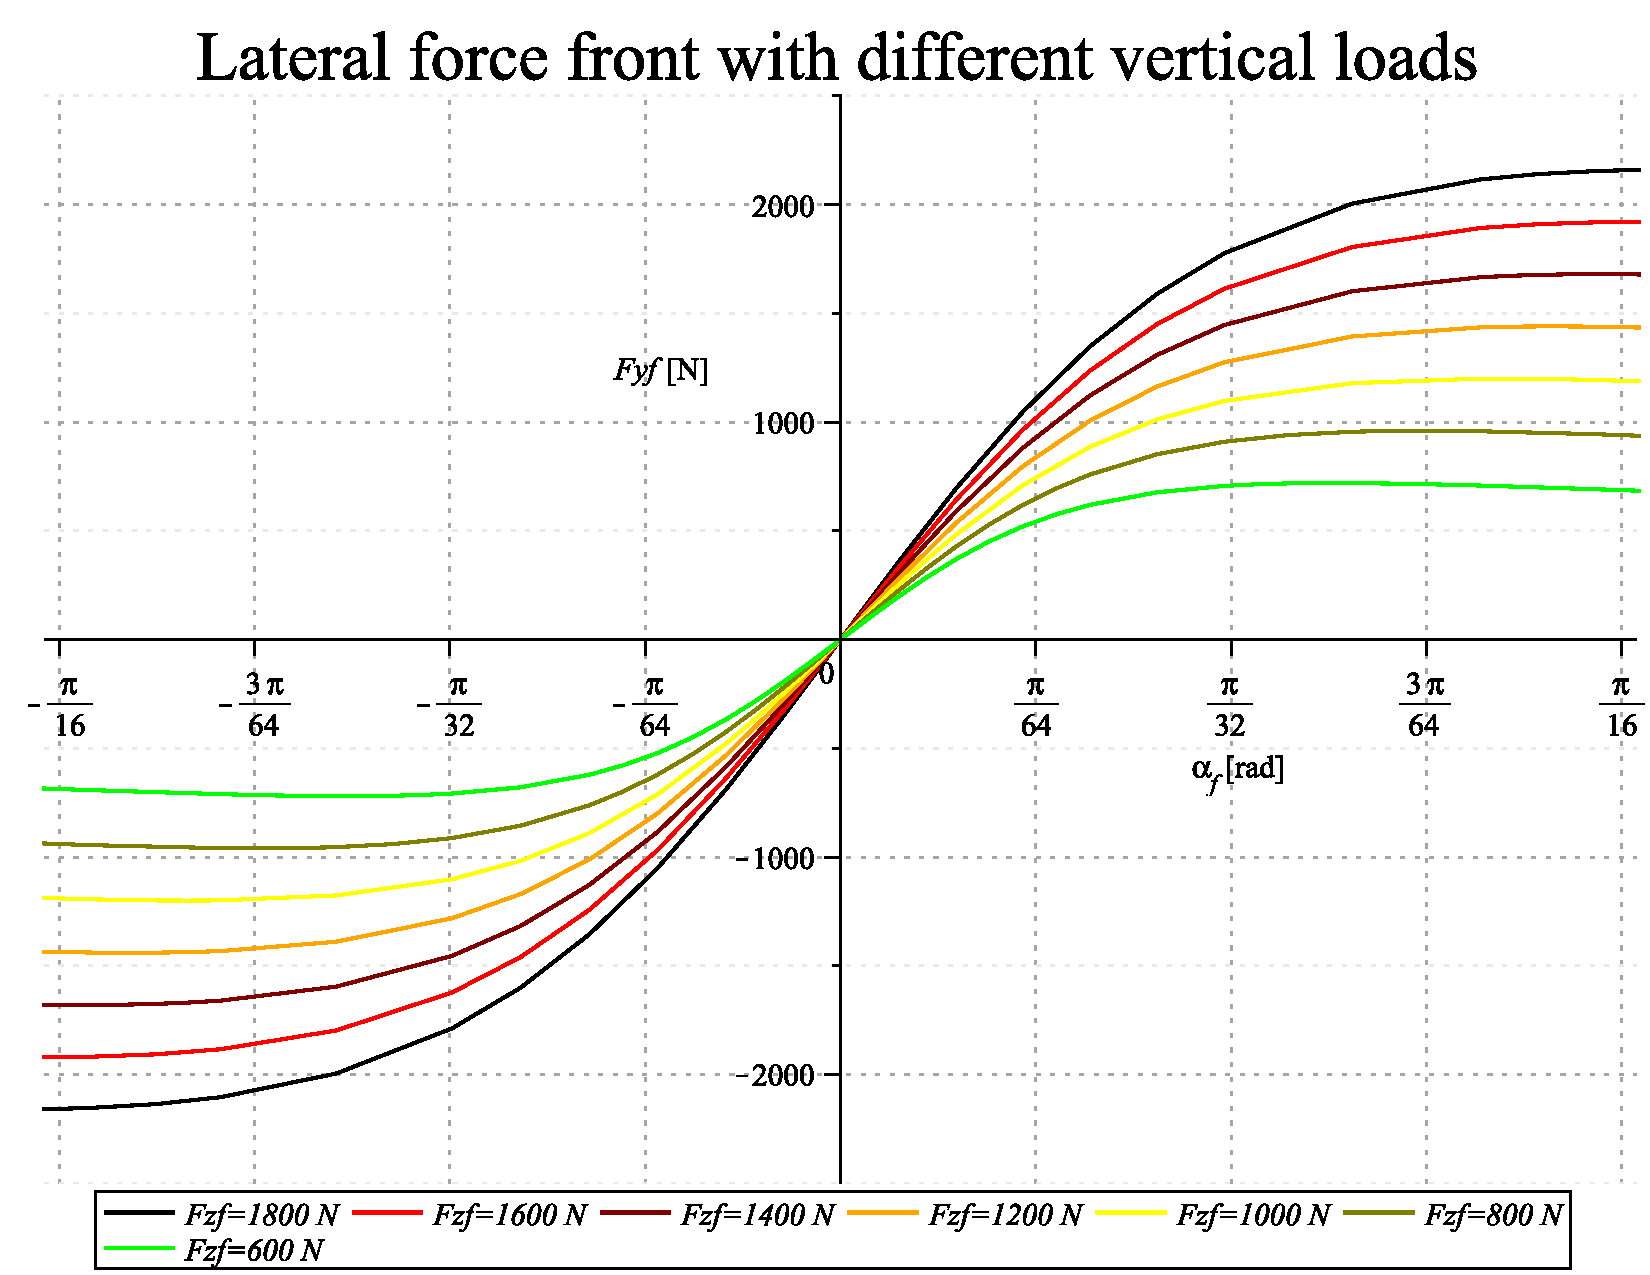
\includegraphics[width=\linewidth]{Pacejka/LatFrontFz.pdf}
        \caption{}
        \label{fig:lat1a}
    \end{subfigure}%
    \begin{subfigure}{.5\textwidth}
        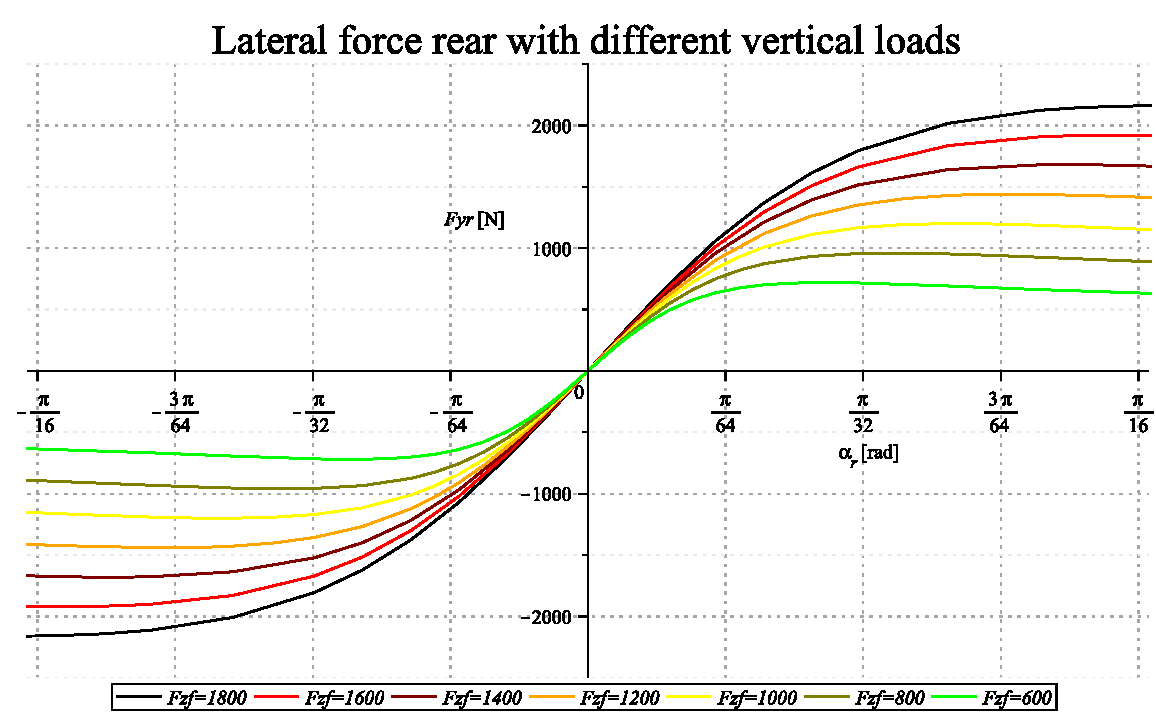
\includegraphics[width=\linewidth]{Pacejka/LatRearFz.pdf}
        \caption{}
        \label{fig:lat1b}
    \end{subfigure}\\
    \begin{subfigure}{.5\textwidth}
        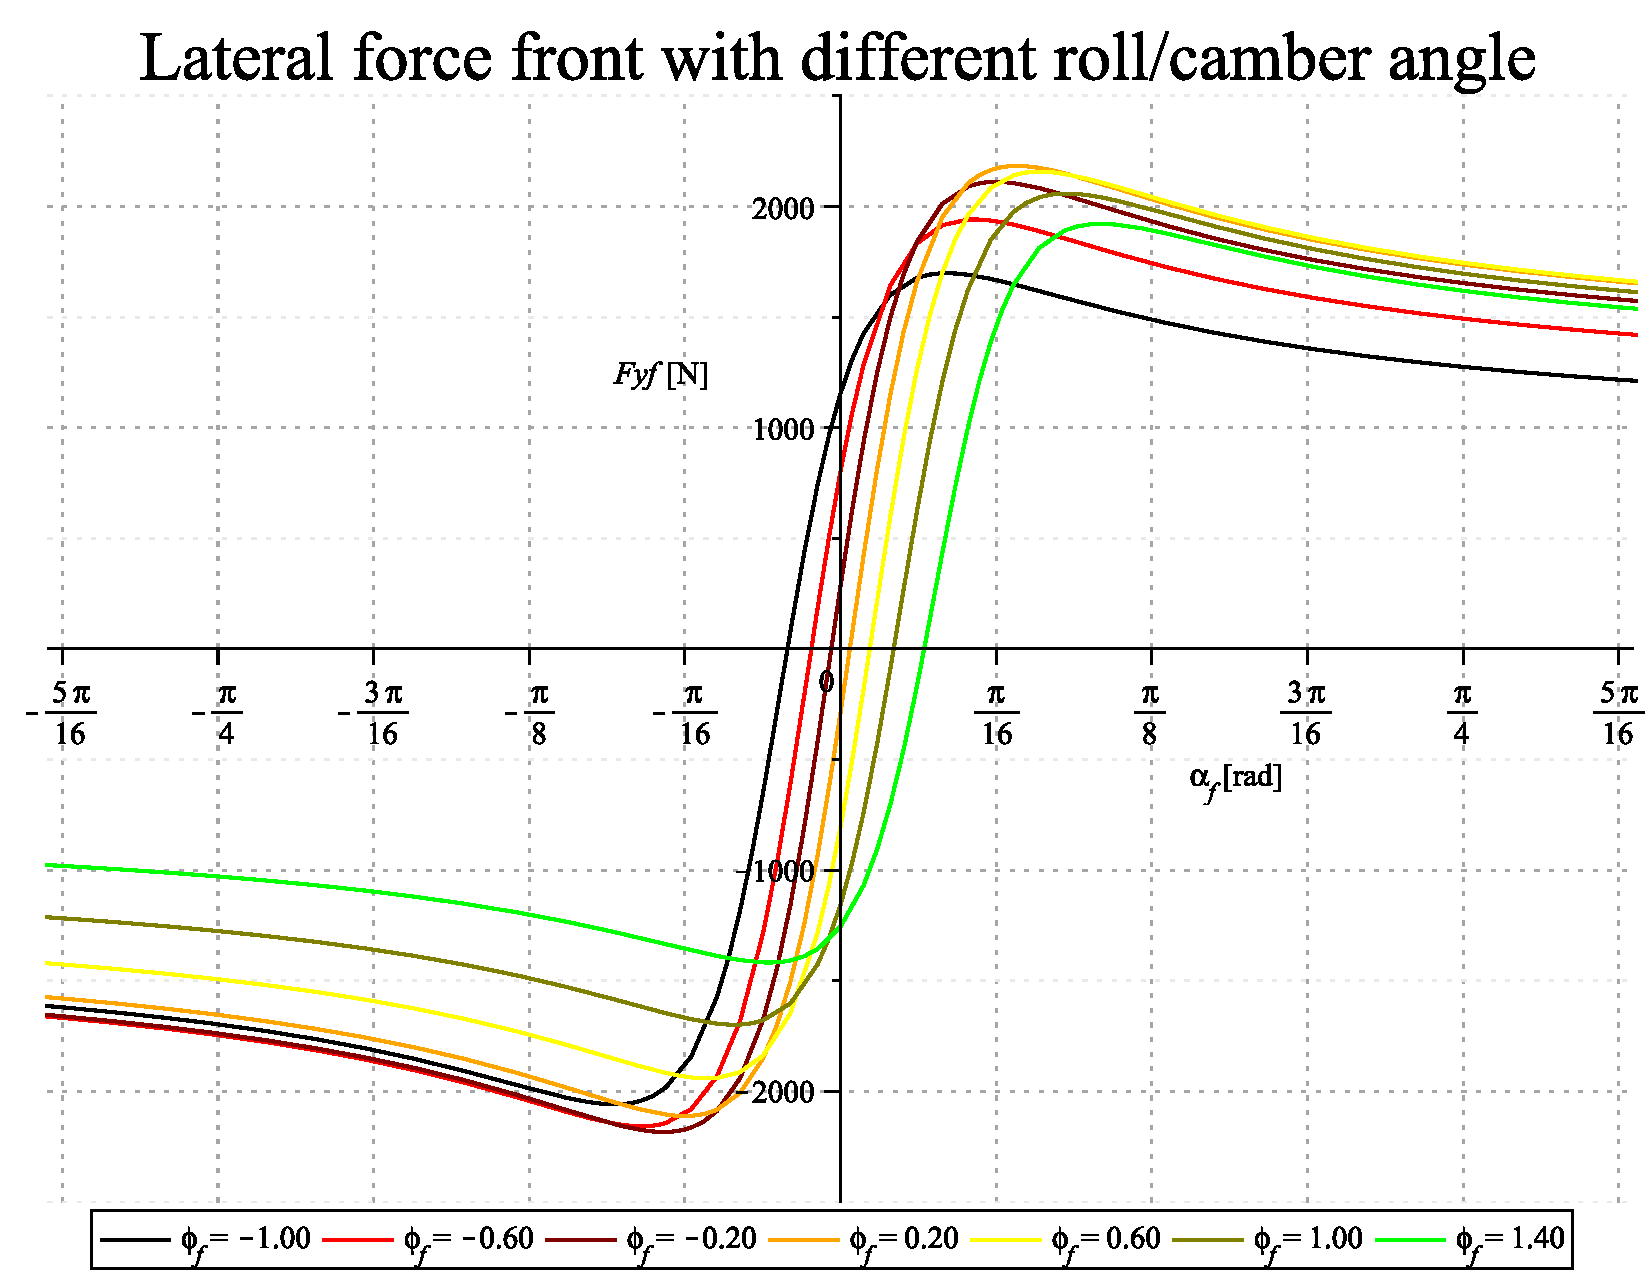
\includegraphics[width=\linewidth]{Pacejka/LatFrontPhi.pdf}
        \caption{}
        \label{fig:lat1c}
    \end{subfigure}%
    \begin{subfigure}{.5\textwidth}
        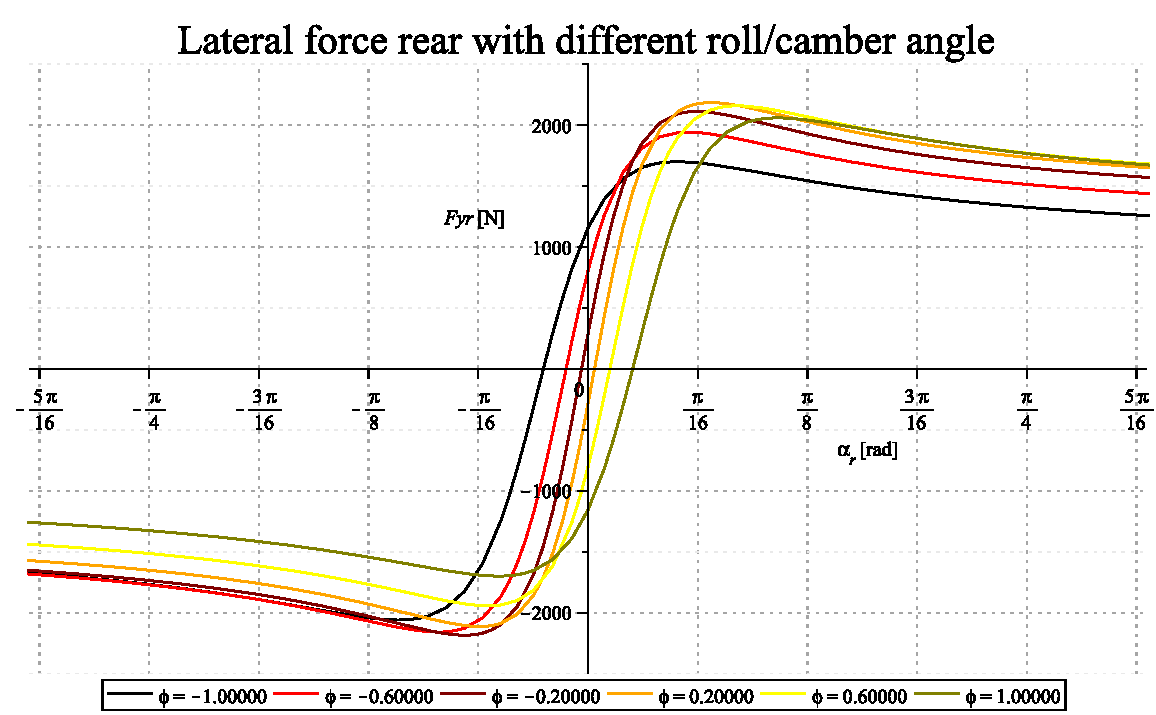
\includegraphics[width=\linewidth]{Pacejka/LatRearPhi.pdf}
        \caption{}
        \label{fig:lat1d}
    \end{subfigure}
    \caption{Graphs of the lateral force for front and rear wheel}
\end{figure}
%
%
The lateral force depends on the lateral slip, namely $\alpha_f$ and $\alpha_r$. They are both function of time even if here the time dependency is dropped out to simplify the notation. In straight motion there is no lateral velocity therefore the lateral slip is null along with the lateral forces. Lateral forces also depends on camber angle that in the case of motorcycle coincide with the roll angle. The rear wheel has a camber angle that is exactly $\phi$ while the front wheel is affected also by the steering angle and therefore his camber is equal to $\phi_f$. 
%
\begin{equation}
    \begin{array}{l}
        Fyf = D_f \sin(C_f \arctan(B_f ( \alpha_{Feq_f} + SH_f))) + SV_f\\
        Fyr = D_r \sin(C_r \arctan(B_r ( \alpha_{Feq_r} + SH_r))) + SV_r
    \end{array}
\end{equation}
%
All coefficient are defined hereafter.
%
% \begin{equation}
%     \left[ \begin {array}{c} {\it Fz}_{f} ={\it Fzf} \left(t \right)
%     \\ {\it CF}_{\alpha_{f}} =\frac{{\it CF}_{\alpha0_{f
%     }} }{{\it d5}_{f} ~\gamma_{f} ^{2}+1}\\ {\it CF}_{
%     \alpha0_{f}} ={\it d1}_{f} ~{\it Fz0}_{f} +{\it d2}_{f} ~\left({\it Fz
%     }_{f} -{\it Fz0}_{f} \right)\\ {\it CF}_{\gamma_{f}}
%      ={\it d3}_{f} ~{\it Fz}_{f} \\ {\it CM}_{\alpha_{f}
%     } ={\it e1}_{f} ~{\it Fz}_{f} \\ {\it CM}_{\gamma_{f
%     }} ={\it e2}_{f} ~{\it Fz}_{f} \\ {\it CMx}_{\gamma_
%     {f}} ={\it e3}_{f} ~{\it Fz}_{f} \\ {\it Fx}_{f} ={
%     \it Fxf} \left(t \right)\\ C_{f} ={\it d8} 
%     \\ K_{f} ={\it CF}_{\alpha_{f}} 
%     \\ {\it D0}_{f} =\frac{{\it d4}_{f} ~{\it Fz}_{f} }{
%     {\it d7}_{f} ~\gamma_{f} ^{2}+1}\\ D_{f} =\sqrt{{
%     \it D0}_{f} ^{2}}\\ B_{f} =\frac{K_{f} }{C_{f} ~{
%     \it D0}_{f} }\\ {\it SHf}_{f} =\frac{{\it CF}_{
%     \gamma_{f}} ~\gamma_{f} }{{\it CF}_{\alpha_{f}} }\\ 
%     {\it SV}_{f} =\frac{{\it d6}_{f} ~{\it Fz}_{f} ~\gamma_{f} ~D_{f} }{{
%     \it D0}_{f} }\\ {\it SH}_{f} ={\it SHf}_{f} -\frac{{
%     \it SV}_{f} }{{\it CF}_{\alpha_{f}} }\\ \alpha_{{
%     \it Feq}_{f}} =\frac{{\it D0}_{f} ~\left(\alpha_{f} -{\it SHf}_{f} 
%     \right)}{D_{f} }-{\it SHf}_{f} \end {array} \right]    
% \end{equation}
% %
% \begin{equation}
%     \left[ \begin {array}{c} {\it Fz}_{r}={\it Fzr} \left( t \right) 
%     \\ {\it CF}_{\alpha_{r}}={\frac {{\it CF}_{\alpha0_{
%     r}}}{{\it d5}_{r}\,{\gamma_{r}}^{2}+1}}\\ {\it CF}_{
%     \alpha0_{r}}={\it d1}_{r}\,{\it Fz0}_{r}+{\it d2}_{r}\, \left( {\it Fz
%     }_{r}-{\it Fz0}_{r} \right) \\ {\it CF}_{\gamma_{r}}
%     ={\it d3}_{r}\,{\it Fz}_{r}\\ {\it CM}_{\alpha_{r}}=
%     {\it e1}_{r}\,{\it Fz}_{r}\\ {\it CM}_{\gamma_{r}}={
%     \it e2}_{r}\,{\it Fz}_{r}\\ {\it CMx}_{\gamma_{r}}={
%     \it e3}_{r}\,{\it Fz}_{r}\\ {\it Fx}_{r}={\it Fxr}
%      \left( t \right) \\ C_{r}={\it d8}
%     \\ K_{r}={\it CF}_{\alpha_{r}}\\ {
%     \it D0}_{r}={\frac {{\it Fz}_{r}\,{\it d4}_{r}}{{\it d7}_{r}\,{\gamma_
%     {r}}^{2}+1}}\\ D_{r}=\sqrt {{{\it D0}_{r}}^{2}}
%     \\ B_{r}={\frac {K_{r}}{{\it D0}_{r}\,C_{r}}}
%     \\ {\it SHf}_{r}={\frac {\gamma_{r}\,{\it CF}_{
%     \gamma_{r}}}{{\it CF}_{\alpha_{r}}}}\\ {\it SV}_{r}=
%     {\frac {D_{r}\,\gamma_{r}\,{\it Fz}_{r}\,{\it d6}_{r}}{{\it D0}_{r}}}
%     \\ {\it SH}_{r}={\it SHf}_{r}-{\frac {{\it SV}_{r}}{
%     {\it CF}_{\alpha_{r}}}}\\ \alpha_{{\it Feq}_{r}}={
%     \frac {{\it D0}_{r}\, \left( \alpha_{r}-{\it SHf}_{r} \right) }{D_{r}}
%     }-{\it SHf}_{r}\end {array} \right]    
% \end{equation}
%
\begin{equation}
    \left[ \begin {array}{c} {\it Fz}_{i} ={\it Fzi} \left(t \right)
    \\ \displaystyle {\it CF}_{\alpha_{i}} =\frac{{\it CF}_{\alpha0_{i
    }} }{{\it d5}_{i} ~\gamma_{i} ^{2}+1}\\ {\it CF}_{
    \alpha0_{i}} ={\it d1}_{i} ~{\it Fz0}_{i} +{\it d2}_{i} ~\left({\it Fz
    }_{i} -{\it Fz0}_{i} \right)\\ {\it CF}_{\gamma_{i}}
     ={\it d3}_{i} ~{\it Fz}_{i} \\ {\it CM}_{\alpha_{i}
    } ={\it e1}_{i} ~{\it Fz}_{i} \\ {\it CM}_{\gamma_{i
    }} ={\it e2}_{i} ~{\it Fz}_{i} \\ {\it CMx}_{\gamma_
    {i}} ={\it e3}_{i} ~{\it Fz}_{i} \\ {\it Fx}_{i} ={
    \it Fxi} \left(t \right)\\ C_{i} ={\it d8} 
    \\ K_{i} ={\it CF}_{\alpha_{i}} 
    \\ \displaystyle {\it D0}_{i} =\frac{{\it d4}_{i} ~{\it Fz}_{i} }{
    {\it d7}_{i} ~\gamma_{i} ^{2}+1}\\ D_{i} =\sqrt{{
    \it D0}_{i} ^{2}}\\ \displaystyle B_{i} =\frac{K_{i} }{C_{i} ~{
    \it D0}_{i} }\\ \displaystyle {\it SHf}_{i} =\frac{{\it CF}_{
    \gamma_{i}} ~\gamma_{i} }{{\it CF}_{\alpha_{i}} }\\ 
    \displaystyle {\it SV}_{i} =\frac{{\it d6}_{i} ~{\it Fz}_{i} ~\gamma_{i} ~D_{i} }{{
    \it D0}_{i} }\\ \displaystyle {\it SH}_{i} ={\it SHf}_{i} -\frac{{
    \it SV}_{i} }{{\it CF}_{\alpha_{i}} }\\ \displaystyle \alpha_{{
    \it Feq}_{i}} =\frac{{\it D0}_{i} ~\left(\alpha_{i} -{\it SHf}_{i} 
    \right)}{D_{i} }-{\it SHf}_{i} \end {array} \right]    
\end{equation}
%
where $i$ is everywhere in place of $r$ or $f$, rear and front wheel.\\
In the previous definitions $\gamma_i$ is actually the camber angle $\phi$ or $\phi_f$ depending on the addressed wheel. The angle $alpha_i$ is the side slip angle and is used to calculate the equivalent side slip $\alpha_{Feq_i}$.\\
In figure \ref{fig:lat1a} and \ref{fig:lat1b} the effect of vertical load $Fz$ on lateral force is show for both wheels. As expected from the model definition, the lateral force scale with the applied load. Figure \ref{fig:lat1c} and \ref{fig:lat1d}, instead, represent the effect of the different chamber angles on lateral loads. It is clear that this angle plays a major role in the range between $-60$ and $60$ degrees. 
%
\section{Self-aligning moment}
%
\begin{figure}%[hbt]
    \begin{subfigure}{.5\textwidth}
        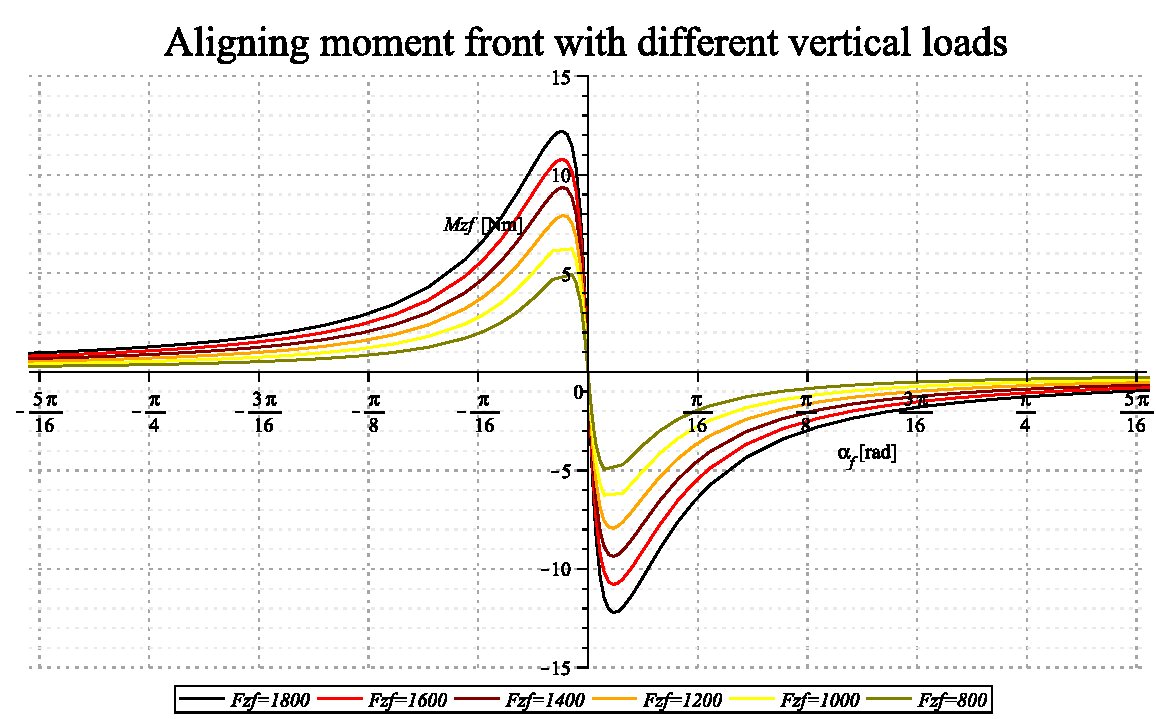
\includegraphics[width=\linewidth]{Pacejka/SelfAliFrontFz.pdf}
        \caption{}
        \label{fig:sa1a}
    \end{subfigure}%
    \begin{subfigure}{.5\textwidth}
        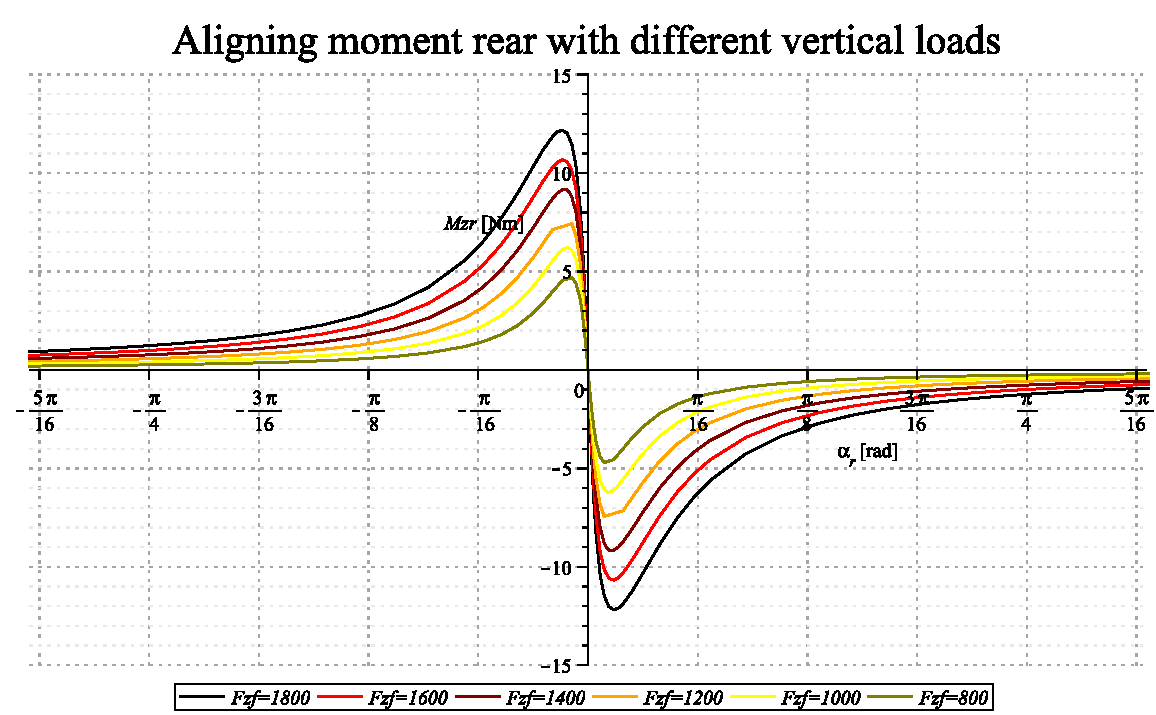
\includegraphics[width=\linewidth]{Pacejka/SelfAliRearFz.pdf}
        \caption{}
        \label{fig:sa1b}
    \end{subfigure}\\
    \begin{subfigure}{.5\textwidth}
        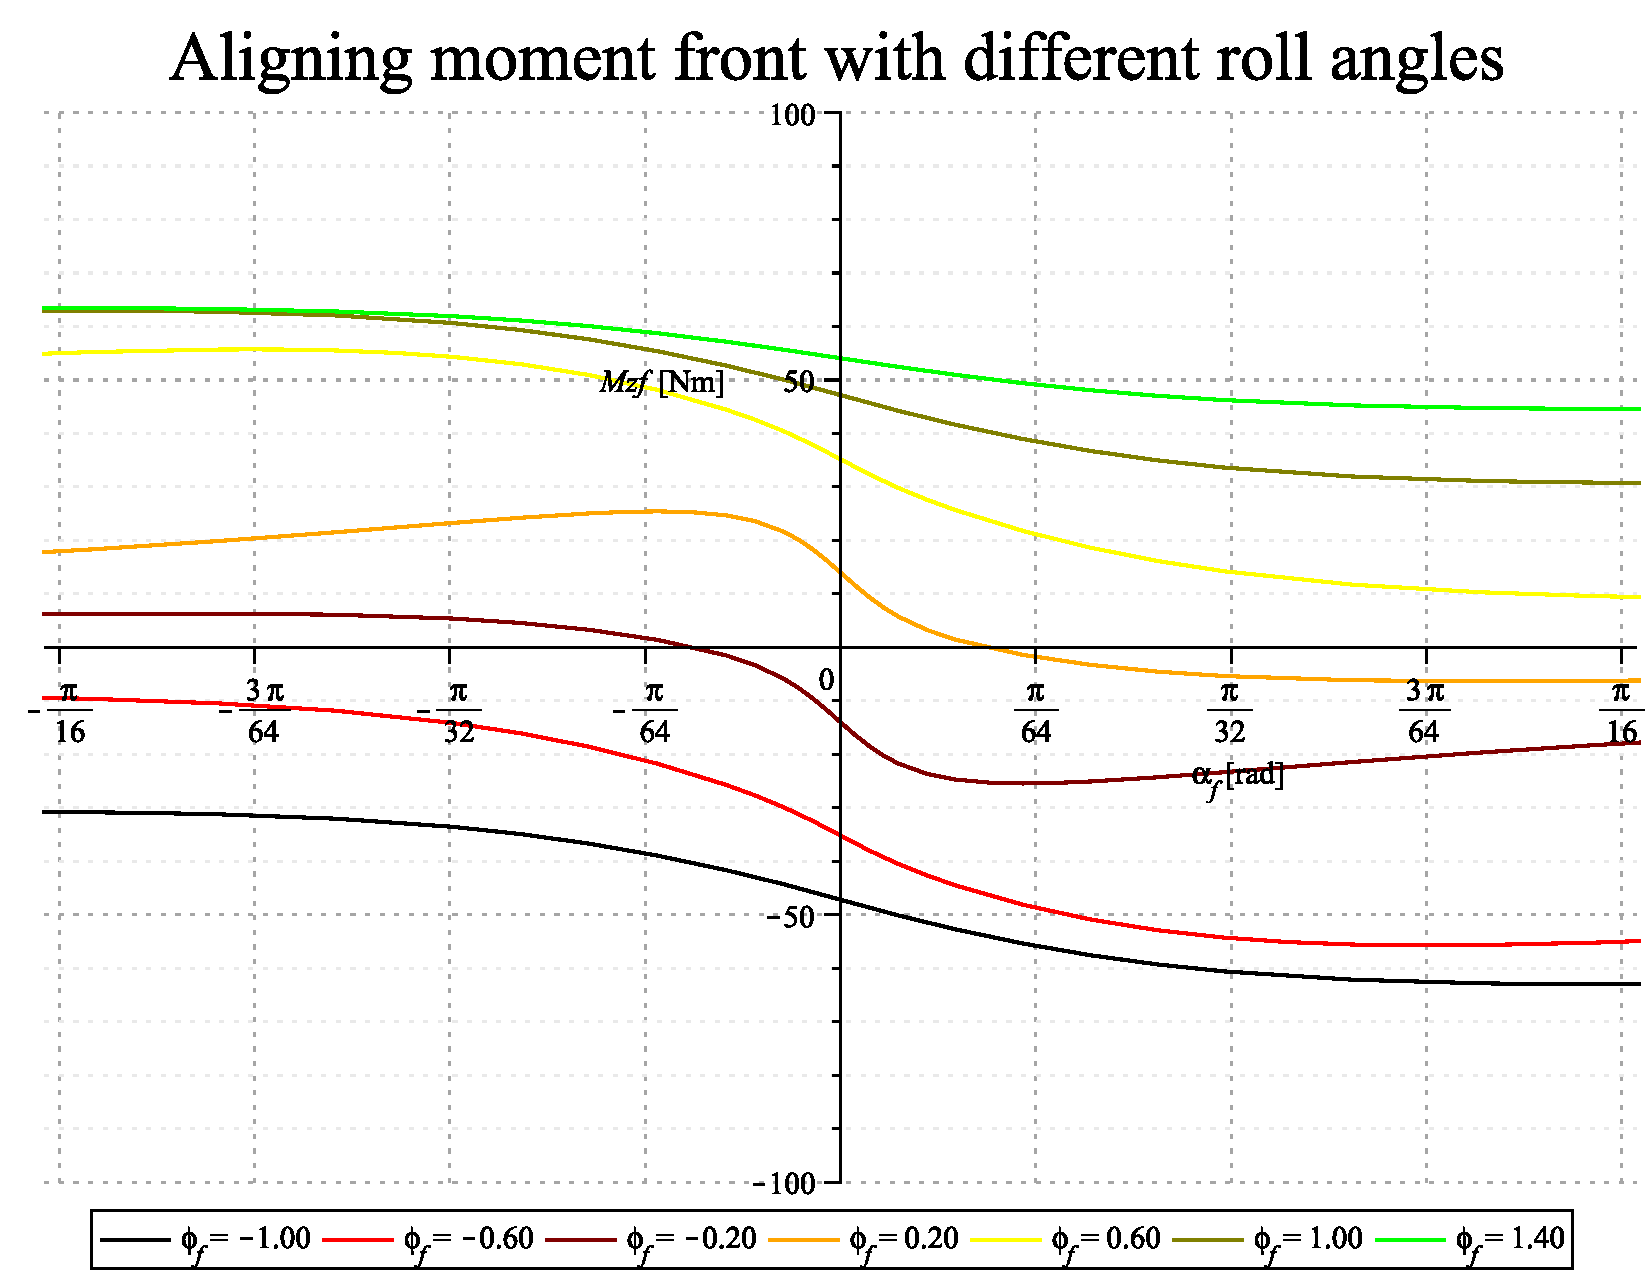
\includegraphics[width=\linewidth]{Pacejka/SelfAliFrontPhi.pdf}
        \caption{}
        \label{fig:sa1c}
    \end{subfigure}%
    \begin{subfigure}{.5\textwidth}
        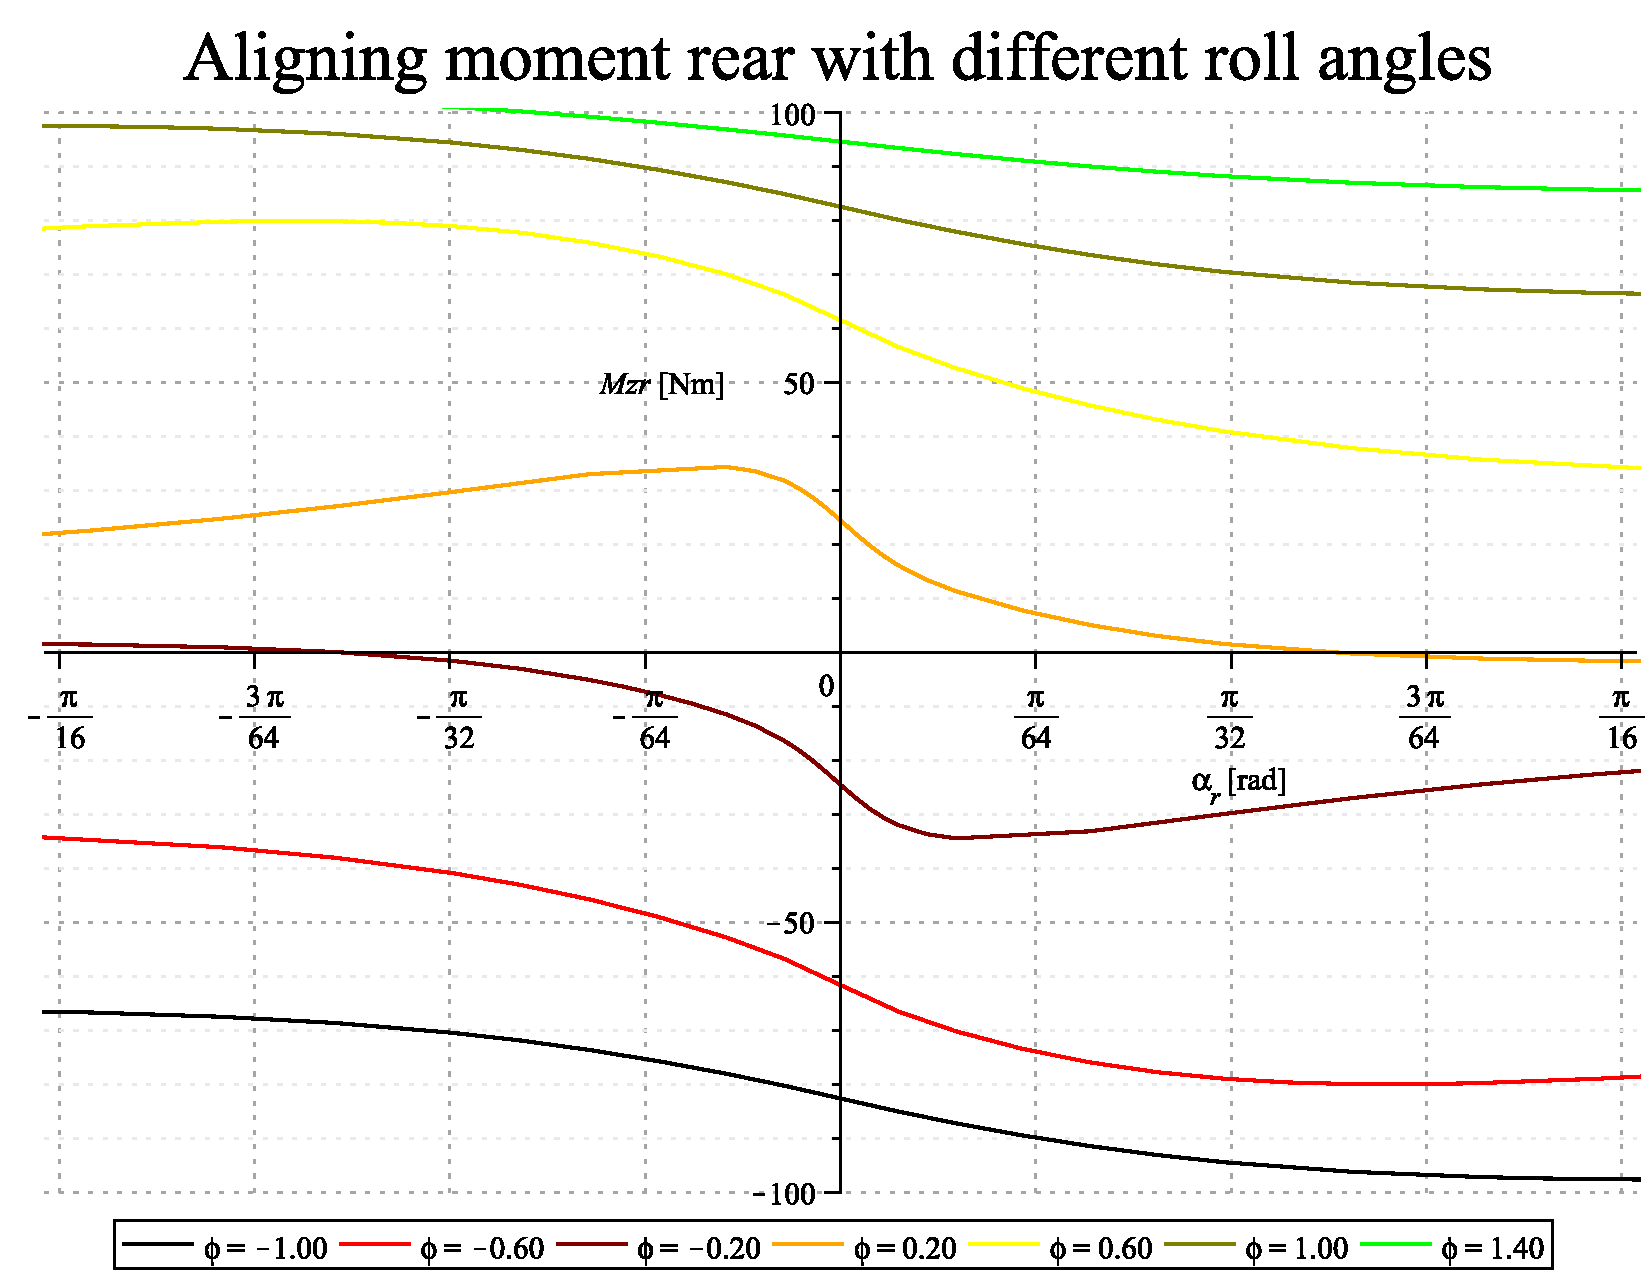
\includegraphics[width=\linewidth]{Pacejka/SelfAliRearPhi.pdf}
        \caption{}
        \label{fig:sa1d}
    \end{subfigure}
    \caption{Graphs of the self-aligning moments for front and rear wheel}
\end{figure}
%
%
The self-aligning moment depends on the lateral slips and chamber angle. As well as fot the other forces previously defined, the time dependency is dropped out to simplify the notation.  
%
\begin{equation}
    \begin{array}{l} 
        {\it Mzf}  =-{\it Fy}_{
        \alpha_{f}}\,t_{\alpha_{f}}+{\it Mzr}_{f}-\tan \left( \gamma_{f}
         \right) {\it Fx}_{f}\,{\it rtf}\\ {\it Mzr} =-{\it Fy}_{\alpha_{r}}\,t_{\alpha_{r}}+{\it Mzr}_{r}-\tan
         \left( \gamma_{r} \right) {\it Fx}_{r}\,{\it rtr}
    \end{array}          
\end{equation}
%
The self-aligning moments depend on three components. The first is the product of the lateral force by a trail ($t$). In fact the lateral force is not acting on the point $P$ defined in chapter \ref{Ch:MotorcycleModel}, this was a modelling expedient. However, there is no such thing as a precise contact point. The force exchange between tyre and ground occurs in a contact patch with an unknown distribution. In fact, this distribution depends on the side slip.\\
The second component of the self-aligning moment depends on the combined effect of chamber and side slip angle. The third therm is an additional torque present because the longitudinal force is not applied in the actual contact point $C$ but in $P$.\cite{pacejka2012tire} \\
All coefficient are defined hereafter.
%
%
% \begin{equation}
%     \left[ \begin {array}{c} t_{\alpha0_{f}} =\frac{{\it CM}_{\alpha_{f}}
%     }{{\it CF}_{\alpha0_{f}} }\\ \alpha_{{\it eq0}_{f}}
%     =\frac{\alpha_{f} ~{\it D0}_{f} }{D_{f} }\\ {\it Fy
%    }_{\alpha_{f}} =\sin \left(\arctan \left(\alpha_{{\it eq0}_{f}} ~B_{f}
%     \right)~C_{f} \right)~D_{f} \\ B_{t_{f}} ={\it e7} 
%    \\ C_{t_{f}} ={\it e8} \\ B_{r_{f}
%    } =\frac{{\it e9} }{\gamma_{f} ^{2}~{\it e4} +1}\\ C
%    _{r_{f}} =\frac{{\it e10} }{\gamma_{f} ^{2}~{\it e5} +1}
%    \\ t_{\alpha_{f}} =\frac{\cos \left(\arctan \left(
%    \alpha_{{\it eq0}_{f}} ~B_{t_{f}} \right)~C_{r_{f}} \right)~t_{\alpha0
%    _{f}} }{\gamma_{f} ^{2}~{\it e5} +1}\\ {\it Mzr0}_{f
%    } =\frac{\arctan \left(\gamma_{f} ~{\it e6} \right)~{\it CM}_{\gamma_{
%    f}} }{{\it e6} }\\ {\it Mzr}_{f} =\cos \left(
%    \arctan \left(\alpha_{{\it eq0}_{f}} ~B_{r_{f}} \right)~C_{r_{f}} 
%    \right)~{\it Mzr0}_{f} \end {array} \right]    
% \end{equation}
% %
% \begin{equation}
%     \left[ \begin {array}{c} t_{\alpha0_{r}}={\frac {{\it CM}_{\alpha_{r}
%     }}{{\it CF}_{\alpha0_{r}}}}\\ \alpha_{{\it eq0}_{r}}
%     ={\frac {\alpha_{r}\,{\it D0}_{r}}{D_{r}}}\\ {\it Fy
%     }_{\alpha_{r}}=\sin \left( \arctan \left( \alpha_{{\it eq0}_{r}}\,B_{r
%     } \right) C_{r} \right) D_{r}\\ B_{t_{r}}={\it e7}
%     \\ C_{t_{r}}={\it e8}\\ B_{r_{r}}=
%     {\frac {{\it e9}}{{\it e4}\,{\gamma_{r}}^{2}+1}}\\ C
%     _{r_{r}}={\frac {{\it e10}}{{\it e5}\,{\gamma_{r}}^{2}+1}}
%     \\ t_{\alpha_{r}}={\frac {\cos \left( \arctan
%      \left( \alpha_{{\it eq0}_{r}}\,B_{t_{r}} \right) C_{r_{r}} \right) t_
%     {\alpha0_{r}}}{{\it e5}\,{\gamma_{r}}^{2}+1}}\\ {
%     \it Mzr0}_{r}={\frac {\arctan \left( \gamma_{r}\,{\it e6} \right) {
%     \it CM}_{\gamma_{r}}}{{\it e6}}}\\ {\it Mzr}_{r}=
%     \cos \left( \arctan \left( \alpha_{{\it eq0}_{r}}\,B_{r_{r}} \right) C
%     _{r_{r}} \right) {\it Mzr0}_{r}\end {array} \right]     
% \end{equation}
%
\begin{equation}
    \left[ \begin{array}{c} 
    \displaystyle t_{\alpha0_{i}} =\frac{{\it CM}_{\alpha_{i}}
    }{{\it CF}_{\alpha0_{i}} }\\ \displaystyle \alpha_{{\it eq0}_{i}}
    =\frac{\alpha_{i} ~{\it D0}_{i} }{D_{i} }\\ {\it Fy
   }_{\alpha_{i}} =\sin \left(\arctan \left(\alpha_{{\it eq0}_{i}} ~B_{i}
    \right)~C_{i} \right)~D_{i} \\ B_{t_{i}} ={\it e7} 
   \\ C_{t_{i}} ={\it e8} \\ \displaystyle B_{r_{i}
   } =\frac{{\it e9} }{\gamma_{i} ^{2}~{\it e4} +1}\\ \displaystyle C
   _{r_{i}} =\frac{{\it e10} }{\gamma_{i} ^{2}~{\it e5} +1}
   \\ \displaystyle t_{\alpha_{i}} =\frac{\cos \left(\arctan \left(
   \alpha_{{\it eq0}_{i}} ~B_{t_{i}} \right)~C_{r_{i}} \right)~t_{\alpha0
   _{i}} }{\gamma_{i} ^{2}~{\it e5} +1}\\ \displaystyle {\it Mzr0}_{i
   } =\frac{\arctan \left(\gamma_{i} ~{\it e6} \right)~{\it CM}_{\gamma_{
   i}} }{{\it e6} }\\ {\it Mzr}_{i} =\cos \left(
   \arctan \left(\alpha_{{\it eq0}_{i}} ~B_{r_{i}} \right)~C_{r_{i}} 
   \right)~{\it Mzr0}_{i} 
    \end{array} \right]    
\end{equation}
%
In figure \ref{fig:sa1a} and \ref{fig:sa1b} the effect of vertical load $Fz$ on self aligning moment is show for both wheels. As expected from the model definition, the peak of the moment scale with the applied load. Figure \ref{fig:sa1c} and \ref{fig:sa1d}, instead, represent the effect of the different chamber angles on the aligning moment. It is clear that this angle plays a major role in the range between $-60$ and $60$ degrees. 
%
\section{Overturning moment}
%
The overturning moment is added to complete the modelling. In fact, as previously highlighted, the force are applied in $P$ both for modelling purposes and for consistence with parameters measurements from literature\cite{pacejka2012tire,sharp2014method}. The overturning moment appears from the translation of the vertical force from $C$ to $P$. Under the assumption of circular cross section of the tyre (torus) the overturning moment is defined as
%
\begin{equation}
    \begin{array}{l} {\it Mxf} \left( t \right) =-{\it Fzf}
    \left( t \right) \tan \left( \phi_{f} \left( t \right)  \right) {\it 
   rtf}\\ {\it Mxr} \left( t \right) =-{\it Fzr}
    \left( t \right) \tan \left( \phi \left( t \right)  \right) {\it rtr}
   \end{array}  
\end{equation}
%
where $rtf$ and $rtr$ are the radii of the toroidal section. In straight condition both chamber angles $\phi$ and $\phi_f$ are null and therefore there is no overturning moment. 
%